

\documentclass[%
12pt,							% Schriftgröße
a4paper,						% Papierformat
oneside, 						% einseitiges (oneside) oder zweiseitiges (twoside) Dokument
listof=totoc, 					% Tabellen- und Abbildungsverzeichnis ins Inhaltsverzeichnis
bibliography=totoc,				% Literaturverzeichnis ins Inhaltsverzeichnis aufnehmen
titlepage, 						% Titlepage-Umgebung statt \maketitle
headsepline, 					% horizontale Linie unter Kolumnentitel
%abstracton,					% Überschrift beim Abstract einschalten, Abstract muss dazu in {abstract}-Umgebung stehen
DIV=12,							% Satzspiegeleinstellung, 12 ist Standar bei KOMA
%BCOR=6mm,						% Bindekorrektur, die den Seitenspiegel um 6mm nach rechts verschiebt,
cleardoublepage=empty,			% Stil einer leeren eingefügten Seite bei Kapitelwechsel
parskip,							% Absatzabstand bei Absatzwechsel einfügen
ngerman
]{scrbook}			
\usepackage{scrhack}			
\usepackage[utf8]{inputenc} 	% ermöglicht die direkte Eingabe von Umlauten
\usepackage[T1]{fontenc} 		% Ausgabe aller zeichen in einer T1-Codierung (wichtig für die Ausgabe von Umlauten!)
\usepackage{babel} 	% deutsche Trennungsregeln und Übersetzung der festcodierten Überschriften
\setlength{\parindent}{0ex} 	% bei neuem Abschnitt nicht einrücken
\usepackage{csquotes}
\usepackage{float}
%------
% Folgende Einstellungen entsprechen den Vorgaben der Leitlinien
\usepackage[onehalfspacing]{setspace}
% Ende Leitlinien
%------
%------
% Folgende Einstellungen sind bei größeren Arbeiten mit viel Text zu empfehlen.
% Hierbei oben DIV=16 einstellen und Zeile \usepackage[onehalfspacing]{setspace} auskommentieren.
%\linespread{1.2}\selectfont     % Zeilenabstand erhöhen - größere Werte als 1.2 nicht verwenden!!
% Ende Einstellung große Arbeiten mit viel Text.
%------

\usepackage{siunitx}			% Vereinfachte Eingabe von Einheiten in Formeln
\sisetup{
	number-unit-product = \;,
	inter-unit-product = \:,
	exponent-product = \cdot,
	output-decimal-marker = {,}
}

\usepackage{graphicx}  			% Einbinden von Grafiken erlauben
\usepackage[format=hang,		% Formatierungen von Unter- / Überschriften
font=normal,
labelfont=bf,
justification=RaggedRight,
singlelinecheck=true,
aboveskip=1mm
]{caption}

\usepackage[backend=biber, %% Hilfsprogramm "biber" beim Compilieren nutzen (statt "biblatex" oder "bibtex")
%style=alphabetic, %% Zitierstil (siehe Dokumentation)
natbib=true, %% Bereitstellen von natbib-kompatiblen Zitierkommandos
hyperref=true, %% hyperref-Paket verwenden, um Links zu erstellen
]{biblatex}
\addbibresource{literature/literatur.bib} %% Einbinden der bib-Datei. Endung .bib unbedingt ergänzen

% Folgende Zeilen sind auszukommentieren, falls runde Klammern und ein vgl. bei Zitaten erscheinen sollen.
%\makeatletter
%\renewcommand{\@cite}[2]{(vgl. {#1\if@tempswa , #2\fi})} 
%\renewcommand{\@biblabel}[1]{(#1)}
%\makeatother

\usepackage{pdfpages}

\usepackage{enumitem}			% Erlaubt Änderung der Nummerierung in der Umgebung enumerate

\usepackage{amsmath}			% Ergänzungen für Formeln
\usepackage{textcomp} 			% zum Einsatz von Eurozeichen u. a. Symbolen
\usepackage{eurosym}			% bessere Darstellung Euro-Symbol mit \euro
\usepackage{tabularx}
\newcommand*\diff{\mathop{}\!\mathrm{d}}	% Differentialzeichen
\newcommand*\Diff[1]{\mathop{}\!\mathrm{d^#1}} % Differentialzeichen höherer Ableitung
\newcommand*\jj{\mathop{}\!\mathrm{j}}	% Komplexe Zahl j

\usepackage[					% Einstellunge Paket hyperref
hyperfootnotes=false			% im pfd-Output Fußnoten nicht verlinken
]{hyperref}

\usepackage{imakeidx}			% Paket zur Erstellung eines Index
\usepackage[intoc]{nomencl} 	% zur Erstellung des Abkürzungsberzeichnisses

\usepackage[					% Einstellungen für Fußnoten
bottom,							% Ausrichtung unten
multiple,						% Trennung durch Seperator bei mehreren Fußnoten
hang,
marginal
]{footmisc}

\usepackage{calc}				% Paket zum Berechnen von Längen z.B. 0.8\linewidth

\usepackage{xcolor} 			% einfache Verwendung von Farben in nahezu allen Farbmodellen

\usepackage{listings}			% Darstellung von Quellcode mit den Umgebungen {lstlisting}, \lstinline und \lstinputlisting
\lstset{literate=				% Damit können Umlaute innerhalb Listings geschrieben werden
	{Ö}{{\"O}}1
	{Ä}{{\"A}}1
	{Ü}{{\"U}}1
	{ß}{{\ss}}1
	{ü}{{\"u}}1
	{ä}{{\"a}}1
	{ö}{{\"o}}1
}
\definecolor{mygreen}{rgb}{0,0.6,0}
\definecolor{mygray}{rgb}{0.5,0.5,0.5}
\definecolor{mymauve}{rgb}{0.58,0,0.82}
\lstset{ %
	backgroundcolor=\color{white},   % choose the background color; you must add \usepackage{color} or \usepackage{xcolor}; should come as last argument
	basicstyle=\footnotesize,        % the size of the fonts that are used for the code
	breakatwhitespace=false,         % sets if automatic breaks should only happen at whitespace
	breaklines=true,                 % sets automatic line breaking
	captionpos=t,                    % sets the caption-position to (b) bottom or (t) top
	commentstyle=\color{mygreen},    % comment style
	deletekeywords={...},            % if you want to delete keywords from the given language
	escapeinside={\%*}{*)},          % if you want to add LaTeX within your code
	escapeinside={(*@}{@*)},
	extendedchars=true,              % lets you use non-ASCII characters; for 8-bits encodings only, does not work with UTF-8
	frame=none,	                   	% "single" adds a frame around the code; "none"
	keepspaces=true,                 % keeps spaces in text, useful for keeping indentation of code (possibly needs columns=flexible)
	keywordstyle=\color{blue},       % keyword style
	language=[LaTeX]TeX,             % the language of the code
	morekeywords={*,nomenclature},   % if you want to add more keywords to the set
	numbers=left,                    % where to put the line-numbers; possible values are (none, left, right)
	numbersep=5pt,                   % how far the line-numbers are from the code
	numberstyle=\tiny\color{mygray}, % the style that is used for the line-numbers
	rulecolor=\color{black},         % if not set, the frame-color may be changed on line-breaks within not-black text (e.g. comments (green here))
	showspaces=false,                % show spaces everywhere adding particular underscores; it overrides 'showstringspaces'
	showstringspaces=false,          % underline spaces within strings only
	showtabs=false,                  % show tabs within strings adding particular underscores
	stepnumber=1,                    % the step between two line-numbers. If it's 1, each line will be numbered
	stringstyle=\color{mymauve},     % string literal style
	tabsize=2,	                   % sets default tabsize to 2 spaces
	title=\lstname                   % show the filename of files included with \lstinputlisting; also try caption instead of title
}

\makeindex						% Indexverzeichnis erstellen
\makenomenclature				% Abkürzungsverzeichnis erstellen

% -----------------------------------------------------------------------------------------------------------------
% Zum Aktualisieren des Abkürzungsverzeichnisses (Nomenklatur) bitte auf der Kommandozeile folgenden Befehl aufrufen :
% makeindex <Dateiname>.nlo -s nomencl.ist -o <Dateiname>.nls
% Oder besser: Kann in TexStudio unter Tools-Benutzer als Shortlink angelegt werden
% Konfiguration unter: Optionen-Erzeugen-Benutzerbefehle: makeindex -s nomencl.ist -t %.nlg -o %.nls %.nlo
% -----------------------------------------------------------------------------------------------------------------

% Hier die persönlichen Daten eingeben:

\newcommand{\titel}{Projektdokumentation Optikerkette SchönesGlas}
%\newcommand{\untertitel}{ggf. Untertitel mit ergänzenden Hinweisen}
\newcommand{\arbeit}{Projektarbeit}
\newcommand{\studiengang}{Fachinformatik}
\newcommand{\studienrichtung}{Anwendungsentwicklung}
\newcommand{\autor}{Malte Blumenthal, Benjamin Schick}
\newcommand{\kurs}{EFI222}
\newcommand{\abgabe}{24.04.2023}
%\newcommand{\betreuerdhbw}{Gutachter der DHBW}
\newcommand{\jahr}{2023}			% für Angabe im Copyright-Vermerk der Titelseite

% Folgende Zeilen definieren Abkürzungen, um Befehle schneller eingeben zu können
\newcommand{\ua}{\mbox{u.\,a.\ }}
\newcommand{\zB}{\mbox{z.\,B.\ }}
\newcommand{\bs}{$\backslash$}

% Folgende Zeilen weden benötigt, um Tikz und PGF-Plot-Grafiken einzubinden
\usepackage{pgfplots}
\usepackage{pgfplotstable}
\pgfplotsset{compat=newest,width=0.6\linewidth}
\usepgfplotslibrary{smithchart}
\usepackage{tikz}						% Tikz sollte nach Listings Pakete geladen werden.
\usetikzlibrary{arrows}

\hyphenation{Schrift-ar-ten}

\begin{document}

	
	\thispagestyle{plain}
\hypersetup{pageanchor=false}
\begin{titlepage}
\enlargethispage{4.0cm}
\sffamily 								% Serifenlose Grundschrift für die Titelseite einstellen
		

\begin{center}

{\fontsize{20.74pt}{24pt}\selectfont
\textbf{\titel}\\[1.5ex]}
{\fontsize{17pt}{20pt}\selectfont
\textbf{\arbeit}\\[2ex]}
{\fontsize{14pt}{17pt}\selectfont
Ausbildung \studiengang\\[2ex]}
{\fontsize{12pt}{14pt}\selectfont
Fachrichtung \studienrichtung\\[1ex]
Elektronikschule Tettnang\\[5ex]
von\\[1ex]
\autor\\[15ex]}

\end{center}

\begin{flushleft}
{\fontsize{12pt}{14pt}\selectfont
\begin{tabular}{ll}
Abgabedatum:					& \quad \abgabe \\
Bearbeitungszeitraum:		   	& \quad 24.03.2023 - 24.04.2023   \\ 
%Matrikelnummer: 				& \quad \matrikelnr \\ 
Klasse: 							& \quad \kurs \\
%Ausbildungsfirma:	 			& \quad \firma \\ 
%Betreuer der Ausbildungsfirma: & \quad \betreuerfirma \\ 

\end{tabular}
}
\end{flushleft}
%%%%% Nachfolgende Zeilen einkommentieren, wenn Copyrightvermerk gewünscht ist
%\begin{flushleft}
%{\fontsize{11pt}{13pt}\selectfont
%Copyrightvermerk:\\
%Dieses Werk einschließlich seiner Teile ist \textbf{urheberrechtlich geschützt}. Jede Verwertung außerhalb der engen Grenzen des Urheberrechtgesetzes ist ohne Zustimmung des Autors unzulässig und strafbar. Das gilt insbesondere für Vervielfältigungen, Übersetzungen, Mikroverfilmungen sowie die Einspeicherung und Verarbeitung in elektronischen Systemen.
%}
%\end{flushleft}
%\begin{flushright}
%{\fontsize{11pt}{13pt}\selectfont \copyright{} \jahr }
%\end{flushright}
\end{titlepage}

\cleardoublepage
\hypersetup{pageanchor=true}
 				
	\pagenumbering{roman}					 
	\tableofcontents
	\cleardoublepage
	\pagenumbering{arabic}
	
	\rmfamily
	\chapter{Projektplanung}
\label{cha:Projektmanagement}

\section{Ausganssituation}
	\subsection{Projektziele}
	\begin{enumerate}
	\item Mobiles ESP8622 \newline
	Als Station für die Aufzeichnung der Daten soll ein Microcontroller verwendet werden. Vorgabe der Stadt Tettnang war ein ESP 8266, welches über eine mobile Stromversorgung betrieben werden soll. 
	Als Sensoren für das Aufzeichnen der Daten sollen ein DHT22 und ein BMP 180 verwendet werden.
	
	\item DHT22 \newline
	Der DHT22 Sensor wird für die Aufzeichnung von Luftfeuchtigkeit und Temperatur verwendet.
	
	\item BMP180 \newline
	Für die Aufzeichnung der Höhe über Normal Null und Luftdruck wird ein BMP180 Sensor verwendet.
	
	\item Raspberry Pi 4 \newline
	Der Webserver braucht Hardware um betrieben zu werden. Da das Verkehrsvolumen auf dem Server als relativ gering eingeschätzt wird, sollte ein Raspberry Pi 4 als Hardwareinfrastruktur ausreichen.
	
	\item Webserver \newline
	Für das Bereitstellen von Visualisierungen der Daten und Aufzeichnung der Daten in einem Datenbank System wird ein Webserver als Interface benötigt. Dafür wird in diesem Projekt NodeJS verwendet.
	
	\item Frontend \newline
	Für die Darstellung der Daten soll eine Website zur Verfügung bereitgestellt werden. Diese soll vorerst eine einzelne Seite sein, die nur eine Tabelle die die Höhe über Normal Null auf einer Horizontalen Zeitachse darstellt.
	
	\item Backend \newline
	Das Backend soll das Topic im MQTT-Broker abonnieren, und dann alle Updates in die Datenbank speichern. Außerdem soll das Backend die Daten aus der Datenbank auslesen und für die Frontendimplementierung bereitstellen.
	
	\item Datenbankserver \newline
	Der Datenbankserver soll auch auf dem Raspberry Pi laufen und die Daten, die von den Sensoren ausgeliefert wurden, permanent abspeichern. Als Datenbanksystem soll MariaDB, eine SQL -Implementierung, verwendet werden.
	
	\item Kommunikation mit MQTT-Broker \newline
	Die Daten müssen zwischen den verschiedenen Geräten ausgetauscht werden. Für die Kommunikation wird im Vorfeld ein öffentlicher MQTT-Broker verwendet. In diesem Projekt wird voraussichtlich mit HiveMQ gearbeitet. Optimal wäre das Hosten eines privaten MQTT-Brokers, aber dies liegt außerhalb des Projektrahmens.
	
	\item Webserver und Broker \newline
	Der Webserver soll sich als Abonnent am entsprechenden Topic des MQTT-Brokers anmelden, um die regelmäßigen Updates des Topics und somit neue Daten zu erhalten.
\end{enumerate}
	\subsection{Teilaufgaben}
	\begin{enumerate}
	\item Festlegung Projektziele
	\item Festlegung Teilaufgaben
	\item Beschreibung Projektumfeld
	\item Beschreibung Projektschnittstellen
	\item Personalplanung
	\item Sachmittelplanung
	\item Terminplanung
	\item Ablaufplan
	\item Kostenplanung
	\item Einrichten Raspberry Pi
	\item Programmierung ESP
	\item Programmierung Backend
	\item Programmierung Frontend
	\item Testen der Infrastruktur mittels Testfahrt
	\item Dokumentation des Pilotprojekts
\end{enumerate}
	\subsection{Projektumfeld, Projektschnittstellen}
	\begin{table} [h]
	\caption{Projektumfeld}
	\begin{tabular}{|l|l|}
		\hline
		Auftraggeber & Elektronikschule Tettnang im Auftrag der Stadt Tettnang \\
		\hline
		Auftragnehmer & Schüler der Klasses EFI222 \\
		\hline
		Räumliches Umfeld & Klassenzimmer an der Elektronikschule Tettnang \\
		\hline
		Ansprechpartner & Herr Rauschmaier \\
		& Frau Wattenbach \\
		& Klassenkameraden \\
		\hline
		Einstieg & Anfrage der Stadt Tettnang \\
		\hline
		Ausstieg & Übergabe des Prototypen \\
		\hline
	\end{tabular}
\end{table}
\section{Ressourcen- und Ablaufplanung}
	\subsection{Terminplanung}
	Gantt Diagramm: siehe Abbildung \ref{fig:terminplanung_gantt} \newline
Tabellarische Darstellung: siehe Abbildung \ref{fig:terminplanung_tabellarisch}

In dieser Zeitplanung sind keine Puffer berücksichtigt worden, da die gesamte Projektzeit sehr knapp bemessen ist.
	\subsection{Personalplanung}
	Die Personalplanung sollte aus der Terminplanung in Abbildung \ref{fig:terminplanung_tabellarisch} sehr offensichtlich hervorgehen.
	\subsection{Sachmittelplanung}
	\begin{table} [H]
	\caption{Sachmittelpanung Hardware}
	\begin{tabularx}{\textwidth}{|l|l|X|l|}
		\hline
		\textbf{Hardware} & \textbf{Menge} & \textbf{Beschreibung} & \textbf{Verfügbarkeit} \\
		\hline
		Entwickler PC & 2x & Hardware benötigt für die Entwicklung der Software und Dokumentation des Projekts & Ist Vorhanden \\
		\hline
		MQTT-Broker (öffentlich) & 1x & MQTT-Server der öffentlich zugänglich ist & Muss beschafft werden \\
		\hline
		Raspberry Pi 4 & 1x & Hardware, welche die Rolle des Servers übernimmt. Ist Host des Webservers und der Datenbank & Muss beschafft werden \\
		\hline
		ESP8266 & 1x & Microcontroller, welcher die Messungen durchführen soll & Muss beschafft werden \\
		\hline
		DHT22 & 1x & Modul für ESP, Zeichnet Temperatur und Luftfeuchtigkeit auf & Muss beschafft werden \\
		\hline
		BMP180 & 1x & Modul für ESP, Zeichnet Höhe über NN und Luftdruck auf & Muss beschafft werden \\
		\hline
	\end{tabularx}
\end{table}
\begin{table} [H]
	\caption{Sachmittelplanung Software}
	\begin{tabularx}{\textwidth}{|l|X|l|}
		\hline
		\textbf{Software} & \textbf{Beschreibung} & \textbf{Verfügbarkeit} \\
		\hline
		Visual Studio Code &  Entwicklungsumgebung für alle Softwareanwendungen, die benötigt werden & Freeware \\
		\hline
		MariaDB & Datenbanksystem, das für das Speichern der Messdaten verwendet wird & Freeware \\
		\hline
		MySQL & Datenbanksprache auf der MariaDB aufbaut & Freeware \\
		\hline
		PlatformIO-Tools & Tools und Bibliotheken für das Programmieren verschiedener Microcontroller & Freeware \\
		\hline
		NodeJS & Webserver für das Hosten von Webanwendungen & Freeware \\
		\hline
		UbuntuServer 22.04 & Betriebssystem für den Server & Freeware \\
		\hline
		C++ & Programmiersprache für ESP8266 & Freeware \\
		\hline
		MQTT & IoT Netzwerkprotokoll & Freeware \\
		\hline
	\end{tabularx}
\end{table}
	\subsection{Kostenplanung}
	\begin{table} [h]
	\centering
	\caption{Kostenplanung}
	\begin{tabularx}{\textwidth}{l c X r}
		\textbf{Artikel} & \textbf{Menge} & & \textbf{Preis} \\
		ESP8622 & 1x & & 8,00 € \\
		Netzteil ESP8622 & 1x & & 5,00 € \\
		Raspberry Pi 4 & 1x & & 50,00 € \\
		Netzteil Raspberry Pi 4 & 1x & & 5,00 € \\
		DHT22 Sensor & 1x & & 10,00 € \\
		BMP180 Sensor & 1x & & 5,00 € \\
		Mobile Stromquelle & 1x & & 15,00 € \\\cline{3-4}
		& & & 98,00 €\\
		& & & \\
		\hline
		Lohn Entwickler & 48x & & 6,00 € \\
		Betriebskosten PC & 2x & & 10,00 € \\\cline{3-4}
		& & & 308,00 € \\
		& & & \\
		\hline
		\textbf{Gesamtpreis} & & & 416,00 € \\\cline{3-4}
		\hline
		\hline
	\end{tabularx}
\end{table}

Somit belaufen sich die geplanten gesamten Projektkosten auf \textbf{416,00\euro{}}.
	\subsection{Qualitätsplanung}
	\begin{itemize}
	\item Qualitätssicherung des Codes mithilfe von GitHub und Versionierung
	\item Regelmäßiger Self-Test der Hardware
	\item Fehlermanagement im Code
	\item SCRUM
	
\end{itemize}
	\chapter{Durchführung- und Auftragsbearbeitung}
\label{cha:Durchfuehrung_und_Auftragsbearbeitung}
\input{sections/03_Einleitung}
\section{ESP8266}
	\subsection{Anschließen der Sensorik}
	Für die Aufgabe wird grundsätzlich nur ein BMP benötigt.
Da jedoch entschieden wurde, die Messdaten um Temperatur und Luftfeuchtigkeit zu erweitern, 
wird ein entsprechender zusätzlicher DHT mit eingebunden.

Da es die Sensoren für den ESP bereits auf entsprechenden Daughterboards angebracht gibt,
war es nur noch nötig diese aufzustecken. \ref{fig:dht_an_esp}
	\subsection{Sensordaten auslesen}
	Weil MicroPython auf dem ESP in Kombination mit einem MQTT-Broker schon 
zuvor im Unterricht Probleme bereitet hat, haben wir uns dazu entschieden, den ESP mit C++ zu programmieren.

Für das Handling der Sensordaten und des Timestamps, welcher später übermittelt werden soll, wurde eine separate Klasse "`sensorData"' \ref{lst:class_sensordata} angelegt.
Über den Konstruktor können die Werte an eine Klasseninstanz übergeben werden. 
Werden diese dann zum Übermitteln an den Broker benötigt, können die Werte dann einfach per Pfeiloperator ("`->"') abgefragt werden.

Für sowohl den DHT als auch den BMP wurde die "`Adafruit\_Sensor"'-Bibliothek verwendet.
Diese wird mit 
\begin{lstlisting}[language=C++]
	#include Adafruit_Sensor.h
\end{lstlisting}
eingebunden.

\subsubsection{Auslesen DHT}
	Beim DHT war es noch zusätzlich notwendig, die "`DHT"'-Bibliothek mit 
\begin{lstlisting}[language=C++]
	#include <DHT.h>
\end{lstlisting}
 	einzubinden.
	Wenn die Bibliothek eingebunden ist, kann eine Instanz vom Typ "`DHT"' und der Bezeichnung "`dht"' mit der Zeile 
\begin{lstlisting}[language=C++]
	DHT dht(02,DHT22);
\end{lstlisting}	
	erzeugt werden.
	Die "`02"' beschreibt den Pin, auf welchen der DHT die Daten sendet und das "`DHT22"' beschreibt den genauen Typ des DHT.
	
	In der Funktion \textit{void setup()} wird mit der Zeile
\begin{lstlisting}[language=C++]
	dht.begin();
\end{lstlisting}
	das Auslesen des Pins gestartet. 
	Jetzt kann in der Funktion \textit{void loop()} mit 
\begin{lstlisting}[language=C++]
	dht.readTemperature();
\end{lstlisting}
	die aktuelle Temperatur und mit
\begin{lstlisting}[language=C++]
	dht.readHumidity();
\end{lstlisting}
	die aktuelle Luftfeuchtigkeit ausgelesen werden.
	
\subsubsection{Auslesen BMP}
	Für den BMP musste noch die "`Adafruit\_BMP085"'-Bibliothek eingebunden werden.
	Hier wurde dann ebenfalls eine Klasseninstanz mit 
\begin{lstlisting}[language=C++]
	Adafruit_BMP085 bmp180;
\end{lstlisting}
	erzeugt. Beim BMP war keine weitere Konfiguration notwendig.
	
	Ähnlich zum DHT wird auch beim BMP das Auslesen mit 
\begin{lstlisting}[language=C++]
	bmp180.begin();
\end{lstlisting}
	in der \textit{void setup()} gestartet.
	Da der Luftdruck jedoch je nach Wetterlage variieren kann, muss der Sensor am Start referenziert werden.
	Da die Höhe des Klassenzimmers bekannt ist (469 m über N.N.), wird immer beim Start mit 
\begin{lstlisting}[language=C++]
	seaLevelPressure = bmp180.readSealevelPressure(currentAltitude);
\end{lstlisting}
	der aktuelle Luftdruck gemessen und auf den Luftdruck auf Meereshöhe rückgerechnet. Dieser wird dann in der Variable "`seaLevelPressure"' gespeichert, welche dann als Referenz für die weiteren Messungen verwendet wird.
	
	Da der BMP mit 
\begin{lstlisting}[language=C++]
	bmp180.readTemperature();
\end{lstlisting}
	ebenfalls die aktuelle Temperatur messen kann, wird aus den Temperaturen des DHT und BMP der Mittelwert gebildet und abgespeichert.
	Die aktuelle Höhe kann über 
\begin{lstlisting}[language=C++]
	bmp180.readAltitude(seaLevelPressure);
\end{lstlisting}
	in Anhängigkeit des zuvor referenzierten Luftdrucks gemessen werden.
	Da auch der Luftdruck auf der Website erscheinen soll, wird dieser mit 
\begin{lstlisting}[language=C++]
	(float)bmp180.readPressure()/100;
\end{lstlisting}
	ausgelesen.
	Die Konvertierung zu einem Float und das Dividieren durch 100 sorgt dafür, dass der Druck in mBar mit Nachkommastellen zurückgeliefert wird.

\subsubsection{Erzeugung Timestamp}
	Da der Timestamp keine zeitliche Abweichung zu den Messergebnissen haben soll, wird dieser annähernd zeitgleich ebenfalls durch den ESP abgespeichert.
	Aufgrund der Tatsache, dass der ESP über keine interne Uhr verfügt und auch 
\begin{lstlisting}[language=C++]
	std::chrono::system_clock::now;
\end{lstlisting}
	nur auf den NTP-Server des verbundenen WLAN-Routers zugreift, kann diese Bibliothek nicht verwendet werden. Wenn der ESP mit dem Hotspot eines Smartphones verbunden wird, liefert 
\begin{lstlisting}[language=C++]
	std::chrono::system_clock::now;
\end{lstlisting}
	nur noch "`0000000000"' zurück, da das Smartphone keinen NTP-Server zur Verfügung stellt.
	Diese Limitierung kann jedoch umgangen werden, indem direkt auf eine URL eines NTP-Servers verwiesen wird, von welchem dann die aktuelle Zeit bezogen werden kann.
	Für den direkten Verweis auf einen NTP-Server sind sowohl die "`NTPClient"' als auch die "`WiFiUdp"'-Bibliothek nötig.
	Die "`WiFiUdp"'-Instanz kann ohne weitere Parameter initialisiert werden:
\begin{lstlisting}[language=C++]
	WiFiUDP ntpUDP;
\end{lstlisting}
	Beim NTPClient müssen die WiFiUdp-Instanz, die URL des NTP-Servers und die Verschiebung zur UTC in Sekunden angegeben werden: 
\begin{lstlisting}[language=C++]
	NTPClient timeClient(ntpUDP, "pool.ntp.org", 7200);
\end{lstlisting}
	Auch der "`timeClient"' muss mit 
\begin{lstlisting}[language=C++]
	timeClient.begin();
\end{lstlisting}
	gestartet werden, jedoch ist hier naheliegenderweise eine WLAN-Verbindung notwendig.
	Bevor die Zeit abgefragt wird, muss der Client mit 
\begin{lstlisting}[language=C++]
	timeClient.update();
\end{lstlisting}
	geupdated werden, dass tatsächlich die aktuelle Zeit zurückgeliefert wird.
	Für einen Timestamp mit Uhrzeit und Datum muss zuerst die "`EpochTime"' abgefragt werden:
\begin{lstlisting}[language=C++]
	timeClient.getEpochTime();
\end{lstlisting}
	Dies liefert einen Unix-Timestamp zurück.
	Dieser kann dann mit 
\begin{lstlisting}[language=C++]
	strftime(timestamp, 20, "`\%Y-\%m-\%d \%H:\%M:\%S"' ,localtime(\&now));
\end{lstlisting}
	in ein YYYY-MM-DD HH:MM:SS Format umformatiert und in die Variable "`timestamp"' abgespeichert werden, wobei die Variable "`now"' die zuvor abgefragte "`EpochTime"' ist.
	
	\subsection{WLAN Verbindung}
	Für die WLAN-Verbindung wurde die "`ESP8266WiFi"'-Bibliothek benötigt.
Der Verbindungsvorgang wurde in eine separate Funktion ausgelagtert, welcher die SSID und das Passwort übergeben werden.\ref{lst:wificonnect}
Diese Funktion wird immer initial in der \textit{void setup()}-Funktion aufgerufen, um die WLAN-Verbindung herzustellen.
Ebenfalls wird bei jedem Durchlauf der \textit{void loop()}-Funktion mit \textit{if(WiFi.status() != WL\_CONNECTED)} überprüft, ob die WLAN-Verbindung noch besteht.
Sollte dies nicht mehr der Fall sein, so wird die Funktion zur Verbindung mit dem WLAN erneut aufgerufen.
	\subsection{Verbinden zu und publishen auf MQTT Broker}
	Um eine Verbindung zu einem (öffentlichen) MQTT-Broker herstellen zu können, wird zusätzlich zur bereits eingebundenen "`ESP8266WiFi"' auch die "`PubSubClient"'-Bibliothek benötigt.
Allerdings ist es nötig, zuerst eine Instanz der Klasse "`WiFiClient"' mit \textit{WiFiClient espClient;} zu erzeugen.
Diese Instanz wird dann wiederum bei der Instanziierung der "`PubSubClient"'-Klasse übergeben: \textit{PubSubClient client(espClient);}.
Auch die Verbindungsherstellung zum MQTT-Broker wurde in eine Funktion ausgelagert.\ref{lst:mqttconnect}
Dieser wird die URL des Brokers sowie der zugehörige Port übergeben.
Die Funktion wird ebenfalls in der \textit{void setup()}-Funktion für die initiale Verbindung aufgerufen, dieser Aufruf erfolgt nachdem die WLAN-Verbindung erfolgreich hergestellt wurde.
Auch beim MQTT-Broker wird bei jedem Durchlauf der \textit{void loop()}-Funktion mit \textit{if(!client.connected())} überprüft, ob die Verbindung noch offen ist um diese gegebenenfalls wiederherzustellen.
Bevor die Messwerte dann an den Broker gepublisht werden können, müssen diese als JSON-Objekt serialisiert werden.
Hierfür wird die "`ArduinoJson"'-Bibliothek eingebunden.
Die Klasseninstanz wird hier mit \textit{JsonDocument serializedData;} nur lokal in der \textit{void loop()}-Funktion erzeugt, sodass dieses in jedem Durchlauf neu erzeugt und am Ende wieder verworfen wird.
Die "`serializedData"'-Instanz wird nun mit den Keys und den enstprechenden Values befüllt.\ref{lst:writejson}
Da jedoch keine Instanz eines JsonDocuments an den MQTT-Broker gepublisht werden kann, muss die Zeichenanzahl bestimmt und der Inhalt zuerst wieder in ein Characterarray gespeichert werden: \textit{size\_t n = serializeJson(serializedData, buffer);}.
Nun können die Messwerte zusammen mit den Keys an den Broker gesendet werden : \textit{client.publish(topic, buffer, n)}.
Hier muss noch die Topic mit angegeben werden, welche dann später wieder vom Server abgefragt werden kann.
Zusätzlich wird der Character Array und die Länge dessen übergeben.
	
\section{Raspberry Pi}
	\subsection{Installation benötigter Software}
	Auf dem Raspberry Pi wurden enstprechend der MariaDB-Server, der NodeJS-Server sowie NPM installiert. NPM wird hier für die Installation von Paketen, welche der NodeJS-Server benötigt, verwendet.
	\subsection{Datenbank}
	\subsubsection{Datenbankplanung}
Als erstes musste ein passendes Datenbankschema entworfen werden, in dem die Sensordaten passend gespeichert werden können. Das folgende Schema stellt die Datenbankstruktur vor.
\begin{figure}[H]
	\centering
	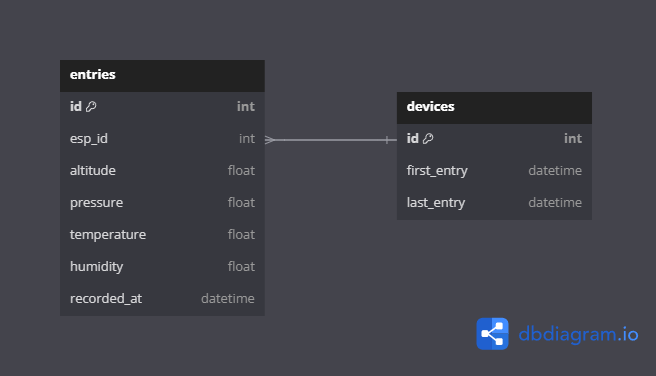
\includegraphics[width=15cm]{images/db_diagram.png}
	\caption{Datenbankdiagramm}
	\label{fig:db_diagram}
\end{figure}
Die Tabelle "`entries"' enthält die Messdaten, Höhe über N.N., den Luftdruck, die Temperatur, die Luftfeuchtigkeit und einen Zeitstempel des Messzeitpunktes, welche das Backend vom MQTT-Broker erhält. Außerdem wurde die Datenbank um eine Tabelle "`devices"' erweitert. Diese Tabelle speichert die einzigartigen Geräte, welche Daten in die Datenbank gespeichert haben. Sie enthält die "`ESP\_ID"' im Feld id, den ersten und letzten Eintrag des Geräts.

\subsubsection{Einrichtung der Datenbank}
Die MariaDB Datenbank wurde durch ein Script initialisiert.  Dieses sollte nur ein einziges mal, vor Inbetriebnahme des Systems ausgeführt werden, da durch Zeile eins, "`DROP DATABASE esp\_data;"', die Datenbank und alle in ihr enthaltenen Daten gelöscht werden. 
\begin{figure}[H]
	\centering
	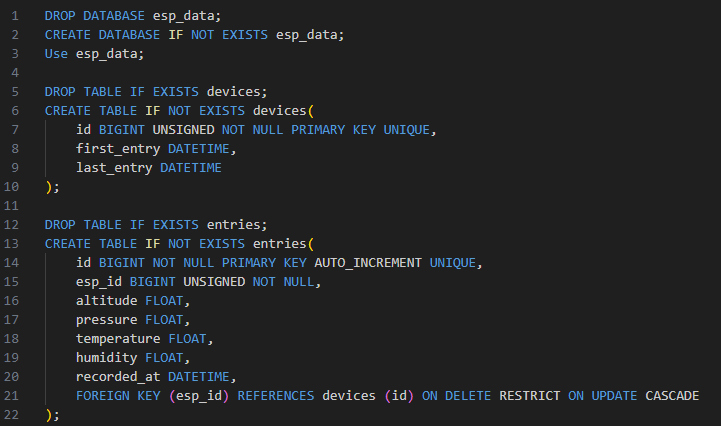
\includegraphics[width=15cm]{images/db_initialisation_script.png}
	\caption{Datenbankinitialisierungsscript}
	\label{fig:db_initialisation_script}
\end{figure}
	\subsection{Programmierung des NodeJS-Servers}
	\subsubsection{Konfiguration der MariaDB Verbindung}
Das folgende Code Snippet bescheibt die Datenbankverbindung zum lokal installierten Datenbankserver. Es enthält die benötigten Bibliotheken, den Userzugang und die Datenbank auf dem Server mit dem sich der Webserver verbindet.
\begin{lstlisting}[language=java]
	//MariaDB
	const mariadb = require('mariadb');
	const pool = mariadb.createPool({
		host: 'localhost',
		user: 'root',
		password: 'toor',
		database: 'esp_data',
		connectionLimit: 2
	});
\end{lstlisting}

\subsubsection{Konfiguration der MQTT Verbindung}
Der folgende Code bescheibt die Konfiguration des MQTT Objekts. Hier wurde nicht, wie geplant, mit HiveMQ gearbeitet, sondern mit Mosquitto. Getestet wurde auch der Eclipseprojects MQTT Broker. Für unser Projekt war aber Mosquitto der stabilste öffentliche Broker. Auch hier werden erst die benötigten Bibliotheken angegeben. Es folgen die Broker-URL, der Port und das Topic. Dann wird eine Verbindung aufgebaut und sich als Abonnent am Topic angemeldet, so dass der Broker Updates an den Webserver schicken kann.
\begin{lstlisting}[language=java]
	//MQTT
	const mqtt = require('mqtt');
	const { each, error, ready } = require("jquery");
	const protocol = 'mqtt';
	const mqtt_broker = 'test.mosquitto.org';
	//const mqtt_broker = 'mqtt.eclipseprojects.io';
	const mqtt_port = 1883;
	const mqtt_url = protocol + '://' + mqtt_broker + ':' + mqtt_port;
	const mqtt_topic = 'est/katastrophenprojekt/espdaten';
	const mqtt_client = mqtt.connect(mqtt_url, keepalive = 60);
	let topic = mqtt_client.subscribe(mqtt_topic);
\end{lstlisting}

\subsubsection{Event: MQTT Message}
Dieses Event beschreibt was passiert, wenn eine Nachricht vom MQTT-Broker empfangen wird. Erst wird die Nachricht in die Konsole geschrieben, was beim Debugging hilft und dann wird die Nachricht in der Funktion: messageRecieved weiterverarbeitet.
\begin{lstlisting}[language=java]
	mqtt_client.on('message', (topic, message) => {
		console.log('Message:' + message);
		messageRecieved(message);
		//console.log('success');
	});
\end{lstlisting}

\subsubsection{Funktion: messageRecieved}
In der Funktion messageRecieved(message) wird, wie oben erwähnt, die Nachricht verarbeitet. Da die Daten in zwei verschiedene Tabellen in der Datenbank geschrieben werden müssen werden hier auch zwei SQL-Queries ausgeführt. 
\begin{lstlisting}[language=java]
	async function messageRecieved(message) {
		let conn;
		let jsonObj = JSON.parse(message);
		try {
			conn = await pool.getConnection();
			const res = await conn.query("INSERT INTO devices (id, first_entry, last_entry) VALUES (?, ?, ?) ON DUPLICATE KEY UPDATE last_entry = VALUES (last_entry);", [jsonObj.device_id, jsonObj.timestamp, jsonObj.timestamp]);
			console.log(res);
			const entry = await conn.query("INSERT INTO esp_data.entries (esp_id, altitude, pressure, temperature, humidity, recorded_at) VALUES (?, ?, ?, ?, ?, ?);", [jsonObj.device_id, jsonObj.altitude, jsonObj.airPressure, jsonObj.temperature, jsonObj.humidity, jsonObj.timestamp]);
			console.log(entry);
		} catch(err) {
			console.log("Error: " + err);
			throw err;
		}
		finally {
			if(conn) return conn.end();
		}
	}
\end{lstlisting}

\subsubsection{Route: getData}
Diese Route wird aufgerufen, wenn die Route: Index geladen wird. Dabei wird die asynchrone Funktion readData(req, res) ausgeführt.
\begin{lstlisting}[language=java]
	app.get("/data", (req, res) => {
		readData(req, res);
	});
\end{lstlisting}

\subsubsection{Funktion: readData}
Die Funktion readData(req, res) liest Daten aus der Datenbank und sendet diese and die Website, damit sie dort visualisiert werden können.
\begin{lstlisting}[language=java]
	async function readData(req, res) {
		let conn;
		try {
			conn = await pool.getConnection();
			data = await conn.query("SELECT * FROM (SELECT * FROM entries ORDER BY recorded_at DESC LIMIT 1000) AS subquery ORDER BY id ASC;");
			res.json(data);
		} catch (err) {
			throw err;
		} finally {
			if (conn) conn.end();
		}
	}
\end{lstlisting}
	\subsection{Programmierung der Website zur Datenvisualisierung}
	Bei der Website wurde Chart.js für die grafische Darstellung der Messwerte benutzt.
Die Messwerte wurden mithilfe der "`fetch"'-API vom Backend angefragt und dann dem zugehörigen Diagramm zugeordnet.
Auf der Website wurden dann vier Diagramme für die Temperatur, Luftfeuchtigkeit, Höhe über N.N. und den Luftdruck angezeigt. \ref{fig:website}
Die Daten werden alle fünf Sekunden neu abgefragt und entsprechend aktualisiert.
	
\section{Knackpunkte, Abweichungen, Anpassungen, Entscheidungen}
	\subsection{Knackpunkte}
	Die Knackpunkte im Projekt sind vorwiegend durch kleinere, jedoch schwer zu lokalisierende Fehler entstanden. \newline

Bei der Datenbank gab es initiale Schwierigkeiten mit dem Initialisierungsskript, welches das Setup und vorwiegend mehrfache Setups stark vereinfacht und beschleunigt.
Letztendlich ließen sich hier die Schwierigkeiten auf inkorrekte Syntax zurückführen, welche jedoch teilweise sehr schwer zu lokalisieren war. \newline
Auch bei der Schnittstelle zwischen der Datenbank und dem NodeJS-Backend gab es aufgrund von Syntaxfehlern mittlere Verzögerungen.
Letztendlich waren wir jedoch in der Lage, alle Fehler zu beheben. \newline
Beim ESP gab es ebenfalls kleinere Startschwierigkeiten, die Verbindung zum Broker konnte anfangs nicht hergestellt werden, was dann jedoch auf einen inkorrekten Port und eine fehlerhafte Klasseninstanziierung zurückzuführen war.
Da der ESP keine interne Zeit hat und seine Zeit immer von einem NTP-Server bezieht gab es auch hier kleinere Umstände.
Da der Hotspot eines Smartphones keinen NTP-Server direkt bereitstellt, musste das Auslesen der Zeit umprogrammiert werden, sodass nicht nur leere Timestamps zurückgeliefert wurden.
	\subsection{Abweichungen}
	Trotz der zuvor erwähnten Komplikationen waren wir in der Lage das Projekt in vollem Umfang noch rechtzeitig fertigzustellen.
Die Einzige Abweichung war der MQTT-Broker. Da HiveMQ nicht stabil zur verfügung stand, wurde ein anderer öffentlicher Broker, Mosquitto, verwendet.
	\subsection{Anpassungen}
	Da wir ausreichend Zeit für etwaige Schwierigkeiten mit eingeplant hatten, mussten keine Anpassungen am finalen Produkt vorgenommen werden.
	\subsection{Entscheidungen}
	Entsprechend der Tatsache, dass es weder Abweichungen noch Anpassungen an der Projektplanung gab, war es nicht vonnöten, Entscheidungen bezüglich möglichen Anpassungen zu treffen.
\section{Qualitätssicherung}
	Hinsichtlich der Qualitätsplanung konnten alle Punkte erfüllt werden.
GitHub wurde von Anfang an für die Versionierung von sowohl Code als auch der Dokumentation verwendet, um immer alles sauber versioniert zu haben. \newline
Auch Self-Tests der Hardware wurden in Form von Überprüfung der Messwerte durchgeführt, diese wurden nur an den MQTT-Broker gepublisht wenn diese nicht NULL waren.\newline
Auch Fehlermanagement im Code wurde betrieben, es wurde regelmäßig auf eine vorhandene WLAN-Verbindung sowie auf eine offene Verbindung zum Broker überprüft, sodass möglichst wenig bis keine Messdaten verloren gehen. \newline
SCRUM wurde in kleinem Stil in Form von regelmäßigen Meetings auch verwendet, so konnten sich die einzelnen Teams austauschen und gegebenenfalls auch entsprechend unterstützen.
	
	\chapter{Projektergebnisse}
\label{cha:Projektergebnisse}

\section{Projektergebnisse}
	\subsection{Abnahme}
	Mit der Abnahme des Projektes sind die Ziele des Kunden für den Rahmen des Projektes vollständig erfüllt worden. Es bestehen trotzdem noch Möglichkeiten das System zu erweitern. Ein Punkt wäre das Layout der Website. Die Website beinhaltet zwar das Impressum, aber dies ist aber auf der „About“- oder „Über Uns“-Seite doch sehr versteckt. Man könnte das Impressum beispielsweise in einen Footer verschieben den man auf allen Seiten sehen kann. Ein weiterer Punkt wäre ein Shopsystem. Dafür müssten die nötigen Anpassungen auf den relevanten Seiten getroffen werden, aber auch die Datenbank müsste für diesen Schritt sehr erweitert werden. Noch dazu kommt, dass das Usermanagement momentan sehr rudimentär implementiert ist, was in einer zukünftigen Version etwa aussehen könnte wie in Abbildung \ref{fig:benutzerspeicherung_datenbank}.

%\begin{figure}[h]
%	\centering
%	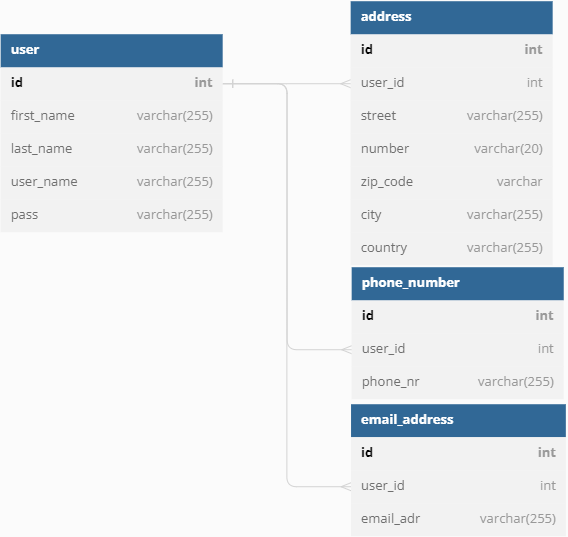
\includegraphics[width=15cm]{images/DatabaseSchemeFuture.png}
%	\caption[Benutzerspeicherung Datenbank]{Benutzerspeicherung in der Datenbank}
%	\label{fig:benutzerspeicherung_datenbank}
%\end{figure}

Der dritte Punkt wäre die Verschlüsselung der Kundendaten. Aktuell wird lediglich das Passwort mit der Methode md5 im Backend, also von Nodejs, gehashed. Das Ziel war ursprünglich alle vom Nutzer eingegebenen Daten im Frontend, also Clientside, zu hashen und zu salten, damit ein potentieller Man-in-the-middle-Angriff sehr viel weniger gefährlich für die Nutzer des Systems und die Optikerkette sind. Man würde durch diese Maßnahme außerdem die Privatsphäre der Nutzer schützen, da keiner der Administratoren die Daten der Nutzer dann willkürlich aus der Datenbank auslesen kann.

	\subsection{Soll-Ist-Vergleich}
	Wie dem Abnahmeprotokoll bereits entnommen werden kann, wurden die Mindestanforderungen erfüllt.
Zusätzlich hierzu können Temperatur und Luftfeuchtigkeit erfasst und auf der Website grafisch dargestellt werden.
	\subsection{Bewertung (Fazit, Ausblick)}
	Sowohl der Code für den ESP als auch der Code von Back- und Frontend können noch optimiert werden.
Aufgrund der zeitlichen Einschränkungen wurde die Funktionalität über Effizienz priorisiert.
Der volle Funktionsumfang ist jedoch gegeben und es gibt keine beträchtlichen Einschränkungen für den Benutzer.
\newline
Der Code könnte sowohl in der Lesbar- und somit auch Wartbarkeit optimiert werden.
Ebenso wäre es im Bereich des Möglichen, noch weitere Funktionen wie beispielsweise einen Login zu integrieren, wodurch die Daten nur noch für autorisierte Personen zugänglich gemacht werden könnten.
	
	\interlinepenalty 10000	
	
	\nocite{*}	
	%\printbibliography	
		
	%\listoffigures
	% alle Abkürzungen, die in der Arbeit verwendet werden. Die Alphabetische Sortierung übernimmt Latex. Nachfolgend sind Beispiele genannt, welche nach Bedarf angepasst, gelöscht oder ergänzt werden können.

% Bei den unten stehenden Formelzeichen ist erläutert, wie explizite Sortierschlüssel über den Inhalt der eckigen Klammer angegeben werden.

% Allgemeine Abkürzungen %%%%%%%%%%%%%%%%%%%%%%%%%%%%
%\nomenclature{Abb.}{Abbildung}
%\nomenclature{bzw.}{beziehungsweise}
%\nomenclature{DHBW}{Duale Hochschule Baden-Württemberg}
%\nomenclature{ebd.}{ebenda}
%\nomenclature{et al.}{at alii}
%\nomenclature{etc.}{et cetera}
%\nomenclature{evtl.}{eventuell}
%\nomenclature{f.}{folgende Seite}
%\nomenclature{ff.}{fortfolgende Seiten}
%\nomenclature{ggf.}{gegebenenfalls}
%\nomenclature{Hrsg.}{Herausgeber}
%\nomenclature{Tab.}{Tabelle}
%\nomenclature{u. a.}{unter anderem}
%\nomenclature{usw.}{und so weiter}
%\nomenclature{vgl.}{vergleiche}
%\nomenclature{z. B.}{zum Beispiel}
%\nomenclature{z. T.}{zum Teil}
\nomenclature{ESP}{Espressif ESP8266}
\nomenclature{MQTT}{Message Queuing Telemetry Transport}
\nomenclature{DHT}{Digital Temperature and Humidity Sensor}
\nomenclature{BMP}{Barometric Pressure Sensor}




% Dateiendungen %%%%%%%%%%%%%%%%%%%%%%%%%%%%%%%%%%%%
%\nomenclature{EMF}{Enhanced Metafile}
%\nomenclature{JPG}{Joint Photographic Experts Group}
%\nomenclature{PDF}{Portable Document Format}
%\nomenclature{PNG}{Portable Network Graphics}
%\nomenclature{XML}{Extensible Markup Language}
\nomenclature{HTML}{Hyper Text Markup Language}
\nomenclature{CSS}{Cascading Style Sheet}
\nomenclature{EJS}{Embedded Javascript Templating}

% Formelzeichen %%%%%%%%%%%%%%%%%%%%%%%%%%%%%%%%%%%%




	
	%% Ggf. folgende Zeile auskommentieren, falls der Sperrvermerk gewünscht ist.
%\chapter*{Sperrvermerk} %*-Variante sorgt dafür, das der Sperrvermerk nicht im Inhaltsverzeichnis auftaucht
%gemäß Ziffer 1.1.13 der Anlage 1 zu §§ 3, 4 und 5  der Studien- und Prüfungsordnung für die Bachelorstudiengänge im Studienbereich Technik der Dualen Hochschule Baden-Württemberg vom 29.09.2017 in der Fassung vom 25.07.2018:
%
%Der Inhalt dieser Arbeit darf weder als Ganzes noch in Auszügen Personen außerhalb des Prüfungsprozesses und des Evaluationsverfahrens zugänglich gemacht werden, sofern keine anders lautende Genehmigung vom Dualen Partner vorliegt.
%
%Musterstadt, den \today \\[4ex]
%
%\rule[-0.2cm]{5cm}{0.5pt} \\
%
%\textsc{\autor} \\[10ex]

\chapter*{Erklärung} %*-Variante sorgt dafür, dass die Erklärung nicht im Inhaltsverzeichnis auftaucht

Wir versichern hiermit, dass wir unsere Dokumentation zur Projektarbeit Projektarbeit mit dem Thema:

\begin{quote}
	\textit{\titel}
\end{quote}

selbstständig verfasst und keine anderen als die angegebenen Quellen und Hilfsmittel benutzt haben. Wir versichern zudem, dass die eingereichte elektronische Fassung mit der gedruckten Fassung übereinstimmt.\\[6ex]

Tettnang, den \today \\[1ex]

\rule[-0.2cm]{15cm}{0.5pt} \\

\autor \\[10ex]

\rmfamily

\thispagestyle{empty}

\cleardoublepage


	
\end{document}